
%\documentclass[letterpaper,english]{article}

\documentclass[10pt,letterpaper,twocolumn,english]{article}

% This fixes the PDF font, whether or not pdflatex is used to compile the document...
\usepackage{pslatex} 

\usepackage[T1]{fontenc}
\usepackage[latin1]{inputenc}
\usepackage{graphicx}
\usepackage{xspace}

\usepackage{geometry,color}
\geometry{verbose,letterpaper,tmargin=1in,bmargin=1in,lmargin=0.75in,rmargin=0.75in}

\makeatletter

\usepackage{babel}

\newcommand{\yad}{LLADD\xspace}
\newcommand{\pin}{loadPage()\xspace}
\newcommand{\unpin}{releasePage()\xspace}
\newcommand{\checkpage}{checkLoaded()\xspace}
\newcommand{\oasys}{Juicer\xspace}

\newcommand{\PP}{\_p\xspace}
\newcommand{\fP}{{$\mathcal P$}\xspace}
\newcommand{\fQ}{{$\mathcal Q$}\xspace}

\newcommand{\eab}[1]{\textcolor{red}{\bf EAB: #1}}
\newcommand{\rcs}[1]{\textcolor{green}{\bf RCS: #1}}
\newcommand{\mjd}[1]{\textcolor{blue}{\bf MJD: #1}}
\newcommand{\jsk}[1]{\textcolor{brown}{\bf JSK: #1}}

%% for space
%% \newcommand{\eab}[1]{}
%% \newcommand{\rcs}[1]{}
%% \newcommand{\mjd}[1]{}

\begin{document}
%\title{\vspace*{-36pt}Application-specific program optimizations\vspace*{-36pt}}
\title{\vspace*{-36pt}Application-specific program optimizations}
\author{Jimmy Kittiyachavalit \and Russell Sears}
\maketitle


%\subsection*{Abstract}


{\em 
Modern software systems are partitioned into modules in order to allow
development efforts to scale gracefully.  Typically, each of these
modules is designed to hide underlying complexity from other software
components, and provides a relatively simple interface so that
programmers that are unfamiliar with the implementation of the module
can reuse it easily. Often, performance is traded for ease of use, as
the client code is unaware of potentials for optimization that the
library's internals present, and the library's implementation can only
implement optimizations that work in the most general case.

In this paper, we describe a source to source code transformation
system that automatically widens an existing library's public
interface, and then uses memoization to implement application specific
optimizations.  We argue that while such a transformation could be
applied manually, doing so would make it difficult to maintain the
library, and would convolute client code, decreasing the usablity of
the system.
}

%\vspace*{-18pt}

\section{Introduction}
\label {intro}

As the size of software systems increase, modularity is typically
introduced in order to reduce the number of potential interactions
between components.  In large systems, this can be a significant
source of inefficiency, since it makes it difficult to implement
optimizations that require tight coupling between the implementations
of the system's interfaces.

One possible solution is to increase the expressivity of the system's
interfaces so that such optimizations are practical, but doing this
undermines the system's modularity by exposing implementation details
in interfaces that are supposed to hide these details.  Another
possibility is to attempt to anticipate typical usage patterns, and
then check for these usage patterns at runtime.  However, checks
placed inside the library must then ignore contextual information that
is easily available to client code.

For example, memoization techniques are commonly employed to store the
results of deterministic function evaluations.  Each time the function
is invoked, its arguments looked up in a data structure.  If the
result is found, it is immediately returned.  If not, then the results
are computed, added to the data structure, and returned.
Unfortunately, the data structure lookup often introduces an
unacceptable amount of runtime overhead.  In cases such as this, a
single pair of arguments and results can be stored in a global, per
library-function variable.  Then, sequential calls with the same set
of arguments will return quickly.  

However, multithreaded software, or software that interleaves
unreleated calls to the same function from many different locations
will not be able to make use of such caching techniques.  In this
work, we store the memoized results in the caller's stack frame,
allowing the number of memoized results to scale with the number of
relevant call sites, and supporting memoization across nested calls to
the same function.

We use \yad, a transactional storage library as a case study.  \yad's
source code contains many calls to \pin and \unpin which look up a
page in an in-memory cache, and fetch the page from disk if necessary.
Profiling a number of \yad's benchmarks revealed that servicing cache
hits was a significant bottleneck, suggesting that \pin should be
optimized.  Therefore, we focus on the \pin function in this work.

\section{Prior work}
\label {prior}

\rcs{We need to look into this!}

\section{System Design}

Optimization of \yad occurs in two phases.  First, the source code is
analysed, functions are transformed so that they take additional
arguments, and a set of sound optimizations are introduced.  The
soundness of the optimizations in this step relies upon the introduction 
of dynamic checks.  At this point, we have produced an optimized, 
compilable version of the original program.

However, the optimized program contains many dynamic checks, and many
of these checks may be unncessary.  This is problematic for two
reasons.  First, it makes it difficult to tell if the optimization
worked as expected without relying on profiling or code coverage tools
to determine whether the dynamic checks succeed at runtime.  This
means it is difficult for programmers to obtain feedback regarding the
quality of the code produced by the optimizer.  In turn, this makes it
difficult for programmers to reason about the implications of changes
to client code, which makes further optimization difficult.  Second,
the dynamic checks have some cost at runtime, and we would like to
minimize this cost.  In the case of \yad, this seems to be neligible.
However, we would like to apply these optimization techniques to other
applications in the future, so it is important that we minimize this
source of overhead.

\subsection{Cil and Dynamic Checks}

We chose to implement a memoization optimization for \yad.  The
optimization is based upon the observation that the return value of a
call to \pin is completely determined by its second argument, a {\em
pageid}.  Furthermore, \yad's calling conventions dictate that
pageid's are passed into functions either as a part of a {\em
recordid} struct, or as an integer named ``page,'' so there is a
simple programmatic way to generate a mapping between arguments to
existing calls and automatically generated Page pointers.

Most functions that take a pageid as an argument either directly or
indirectly \pin the corresponding page.  Therefore, we add an
argument, {\em\PP} to any functions that are passed a pageid, but are
not passed a Page pointer.  At runtime, this argument effectively
proivdes access to one memoized result per call site of the
function.

In the simplest version of the transformation, when the function calls
\pin on the page, it first checks to see if \PP points to the
appropriate page.\footnote{This is done by reading the ``id'' field of
the Page struct referenced by the pointer.  We arrange for these
pointers to either point to a valid Page struct, or to be NULL.}  If
so, it uses \PP instead of calling \pin.  Otherwise, it proceeds as
normal.  If it skips the call to \pin, it remembers that it should
also skip the corresponding call to \unpin.  (See
Figure~\ref{fig:dynamicCheck} for a concrete example of the
transformation.)

Of course, we cannot expect the program to behave correctly unless we
update the call sites of the transformed functions.  When updating
call sites, we distinguish between cases where the caller already has
a page pointer handy, and cases where the caller has no page pointer
in its stack frame.  In the case where a page pointer already exists,
we simply pass the pointer to the child function.

If the caller has no page pointer on its stack, the situation is a bit
tricky.  We could pass the address of a page pointer into the child
function, allowing it to overwrite the caller's page pointer with a
more ``interesting'' one.  However, it is unclear how such an
``interesting'' pointer would be defined, especially since this
pointer would be shared by multiple child functions.  Also, we would need
to create a second clone of each function so that a pointer to a
pointer could be passed in.  

Instead, we opt for a simpler solution, and fall back on the heuristic
that the pageid passed into the child is probably a reasonable choice.
We simply add a Page pointer to the caller's stack frame, and then
call \pin to initialize it to the pageid that is being passed into the
child function.  In order to handle loops, we check that we are
passing in the appropriate Page pointer at each call to a child
function, and call \pin to load a new page if necessary.  The
transformation also arranges for \unpin to be called as appropriate.

In results not presented here, we found that this simple
transformation performed very well on the ``raw read'' benchmark
presented in Section~\ref{codePerformance} but that it was not able to
significantly improve performance for the hash table workload.  It
turns out that this transformation is not very efective on functions
that take a recordid as an argument, but pass a different recordid
into child functions, since they pass \PP into their children
functions, but \PP is probably assoicated with with the wrong pageid.
Therefore, each child must call \pin on the appropriate page. 

Unfortunately, this scenario is relatively common, especially in
implementations of transactional structures that involve levels of
indirection, such as trees or hashtables.  A simple solution to this
problem is to add a new Page pointer to functions that take \PP as an
argument, and pass a pageid to child funcitons.  Then \pin is called
to preload the page, just as it would have been if the \PP argument
did not exist, except that \PP is reused when appropriate.

One final transformation is applied in anticipation of the removale of
dynamic checks described in the next section.  A copy is made of each
function that was modified to take a \PP argument.  We call the
original modified version the ``\fP'' version of the function, and the
new copy the ``\fQ'' version.  The \fQ variant will assume that their caller
passed in a value of \PP that matches the pageid that is passed in.
At this point during optimization, the \fP and \fQ variants are
identical; the only difference is in the semantics of the API they
expose to their callers.  This transformation is in anticipation of
the next phase of optimization, which will remove unnecessary dynamic
checks from the optimized code.

\subsection{Instrumenting for Blast}
\label{instrumenting}
Blast is a static analysis tool that checks code for conformance to a
well defined API.  In order to use it to verify the soundness of our
optimizations, we express the optimizations' soundess in terms of
simple invariants, and then encode these invariants in the transformed
source as calls to API functions.  We then use Blast to check that
these API calls are safe.  If it is able to verify the safety of the
calls, then we know that the optimization is sound.  

In an ideal world, this would mean that we could simply create a new,
dummy function, \checkpage, and insert a call to \checkpage
after each dynamic check introduced above.  We could give the
following spec file to Blast:

\begin{verbatim}
event { 
  pattern { $1 = loadPage($2); }
  action { $1->id = $2; }
}
event { 
  pattern { checkLoaded($1, $2); }  
  guard { $1->id == $2 }
}
\end{verbatim}

Then, we would have Blast verify that each use of \checkpage is safe.
We could then iteratively remove dynamic checks, and have Blast
re-verify the file, as we describe in Section~\ref{delta}.
Unfortunately, this straightforward approach places too much burden on
Blast, especially since we invoke it as part of a larger iterative
process.  Therefore, we had to perform a number of simplifications
before proceeding.

\subsubsection{Pointer Aliasing}

The guard in the original spec file dereferences the page pointer
passed into \checkpage, which means that Blast must consider pointer
aliasing before verifying that \checkpage is called correctly.
Furthermore, the original implementation of \pin is non-trivial, and
ultimately allows aliasing between pointer to different pages unless
\unpin is called correctly.  Also, Blast's pointer analysis is
flow-insensitve.  We found that each of these factors was sufficient
to prevent verification from succeeding even on seemingly 'trivial'
functions.  

Fortunately, according to \yad's API, the Page structure's id field is
never written to outside of \pin and \unpin, and will never be written
to if a function has pinned a page.  Because \pin and \unpin are
designed to behave correctly regardless of the order
in which they are called,\footnote{\unpin could misbehave if called on
an invalid pointer, but we do not remove dynamic checks that surround
\unpin.} we are willing to assume these invariants hold.  Therefore,
in the optimizied source code that we give to Blast, we redefine
\pin as follows:

\begin{verbatim}
Page * loadPage(int pageid) {
  return pageid;
}
\end{verbatim}
Similary, the spec file is changed to this:
\begin{verbatim}
event { 
  pattern { $1 = loadPage($2); }
  action { $1 = $2; }
}
event { 
  pattern { checkLoaded($1, $2); }  
  guard { $1 == $2 }
}
\end{verbatim}

Note that these changes prevent the program from behaving properly.
We are able to perfrom this transformation because we will never
actually compile this variant of the code, and because (given our
assumptions) it does not affect the soundness of Blast's analysis.  We
will use similar tricks throughout the rest of this section.

\subsubsection{Call Graph Simplification}

The next step in preparing the code for verification by Blast is to
reduce the amount of code that must be consider per optimization task.
We achieved this by replacing each call to a \fP or \fQ function with
statements that non-deterministically assign a value to the variables
that could be affected by the original function call.  In the case of
calls to \fQ variants, we also add a \checkpage call to make sure that
the function is properly invoked.\footnote{Initially, no calls to \fQ
variants exist.  Instead, they are added as we iteratively run Blast.}

\subsubsection{Control Flow Graph Simplification}

We found that Blast was usually able to process verification requests
over the simplified callgraph, but certain requests took tens of
minutes to complete or fail.  Upon inspecting the translated code, we
noticed that the follwing call pattern was extremely common:

\begin{verbatim}
if(!p) { 
  ...
  p = loadPage(id);
  ...
} else if(p'->id == id) {
  ...
  p = p';
  ...
} else {
  p = loadPage(id);
}
some_p_variant(p, id);
\end{verbatim}

Blocks such as this are created when the optimizer decides to
speculatively load a page before passing it into a child function.
They have two interesting properties.  First, all possible evaluations
of the large if statement ensure that p->id == id, implying that the
\fP variant at the bottom of the block can be automatically replaced
by a call to an \fQ variant.  Therefore, we can replace all such calls
before passing the program to the iterative Blast evaluator, reducing
the number of sites that we consider when replacing \fP variants with
\fQ variants.

Second, since the block is the result of the optimizers decision to
speculatively load a page for a child function, it is probably not
redundant.\footnote{There are a number of scenarios where this is not
the case, particularly within the bodies of \fQ variants of functions.
We leave the removal of such dynamic checks to future work.}
Therefore, we collapse the conditional into into a single call to
\pin, simplifying the control flow graph of the optimized code
significantly.  

This simplificition, when combined with the ones described above,
reduces the vast majority of Blast runs to under fifteen seconds, with
a small number of calls taking up to one minute.  Due to the call graph
simplification described above, we are able to optimize function calls
independently.  This allows the iterative algorithm described below to
be feasible, reducing the time to optimize the entire library using
naive search to less than an hour.

\section{Removing Dynamic Checks}
The goal of this phase in the transformation is to reduce the overall
execution time of the source program by removing the dynamic checks
introduced earlier.  From this formulation of the problem, it is clear
that not all dynamic checks are created equal; some dynamic checks are
located in code points that are much more frequently executed than
others.  Ideally, we would be able to assign a weight to each dynamic
check proportional to some measure of its run time cost, and then try to
remove a subset of all dynamic checks that minimizes the weight of the
dynamic checks that are remain.  However, we decided that for this
initial implementation, it would be sufficient to assign each of the
dynamic checks equal weight, greatly simplifying the search.  In
addition to assigning each dynamic check the same weight, we made the
assumption that dynamic checks are independent of each other.  That is,
removing one dynamic check will not affect whether or not a different
dynamic check can be removed soundly.  

In order to tell whether a given set of dynamic checks can be removed
soundly, we turn to Blast.  First, we ask Blast to verify that the code
is sound with all the dynamic checks in.  After this, we interatively
search by changing the set of removed checks, and running the resulting
code through Blast.  As an example, consider the following naive search
algorithm used for the numbers cited in this paper \footnote{With the
assumption that all dynamic checks are independent and that all dynamic
checks have equal weight, this naive search finds the optimal solution.}

\begin{verbatim}
for each dynamic check $d in the program $P
    remove $d from $P
    run Blast on $P
    if Blast cannot verify $P as sound
        restore $d in $P
\end{verbatim}


\section{Evaluation}

In this section, we focus on two aspects of the optimization's
behavior.  First, we measure the performance of the transformed code
(before the dynamic checks have been removed).  Second, we measure the
number of checks that Blast is able to remove from the code.  This
second metric measures the quality of feedback that the optimization
provides for the user.

\subsection{Performance of Optimized Code}
\label{codePerformance}
\begin{figure*}[t]
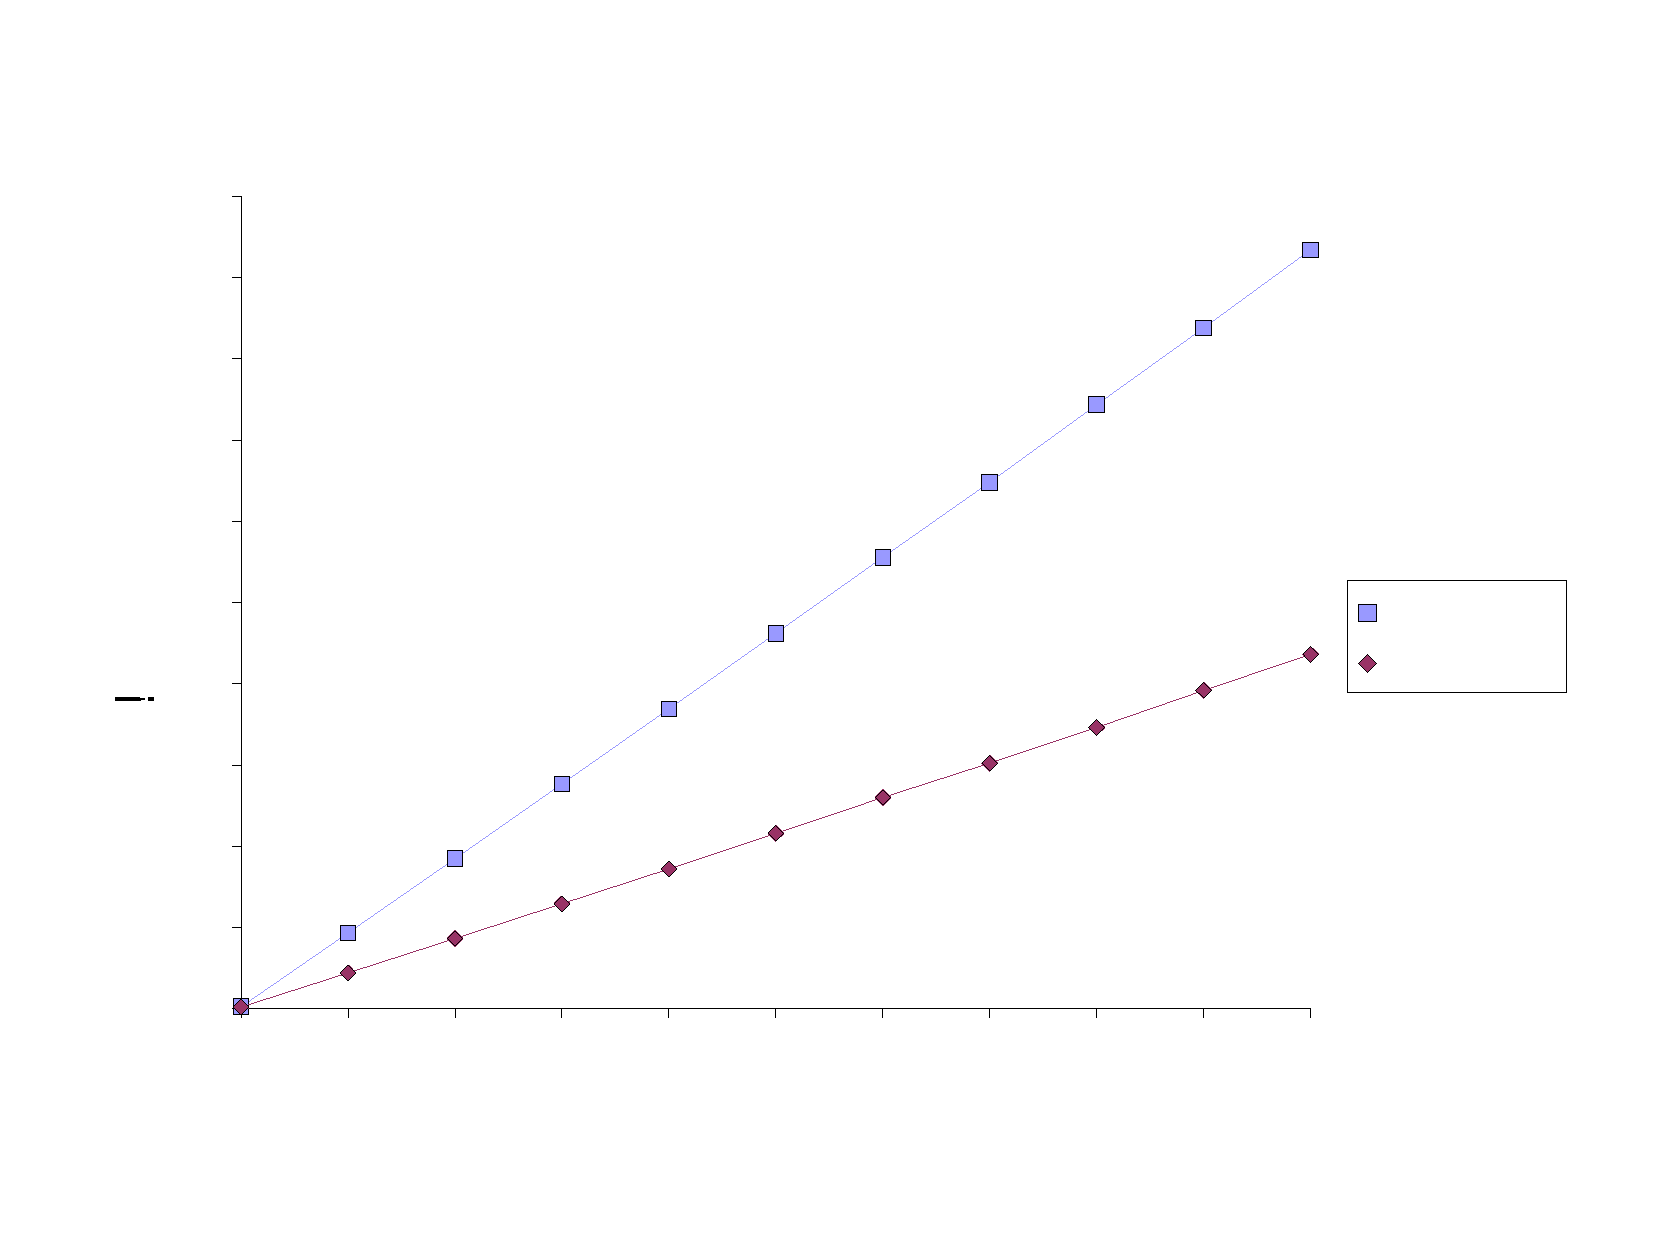
\includegraphics[%
   width=1\columnwidth]{rawReadGraph.pdf}
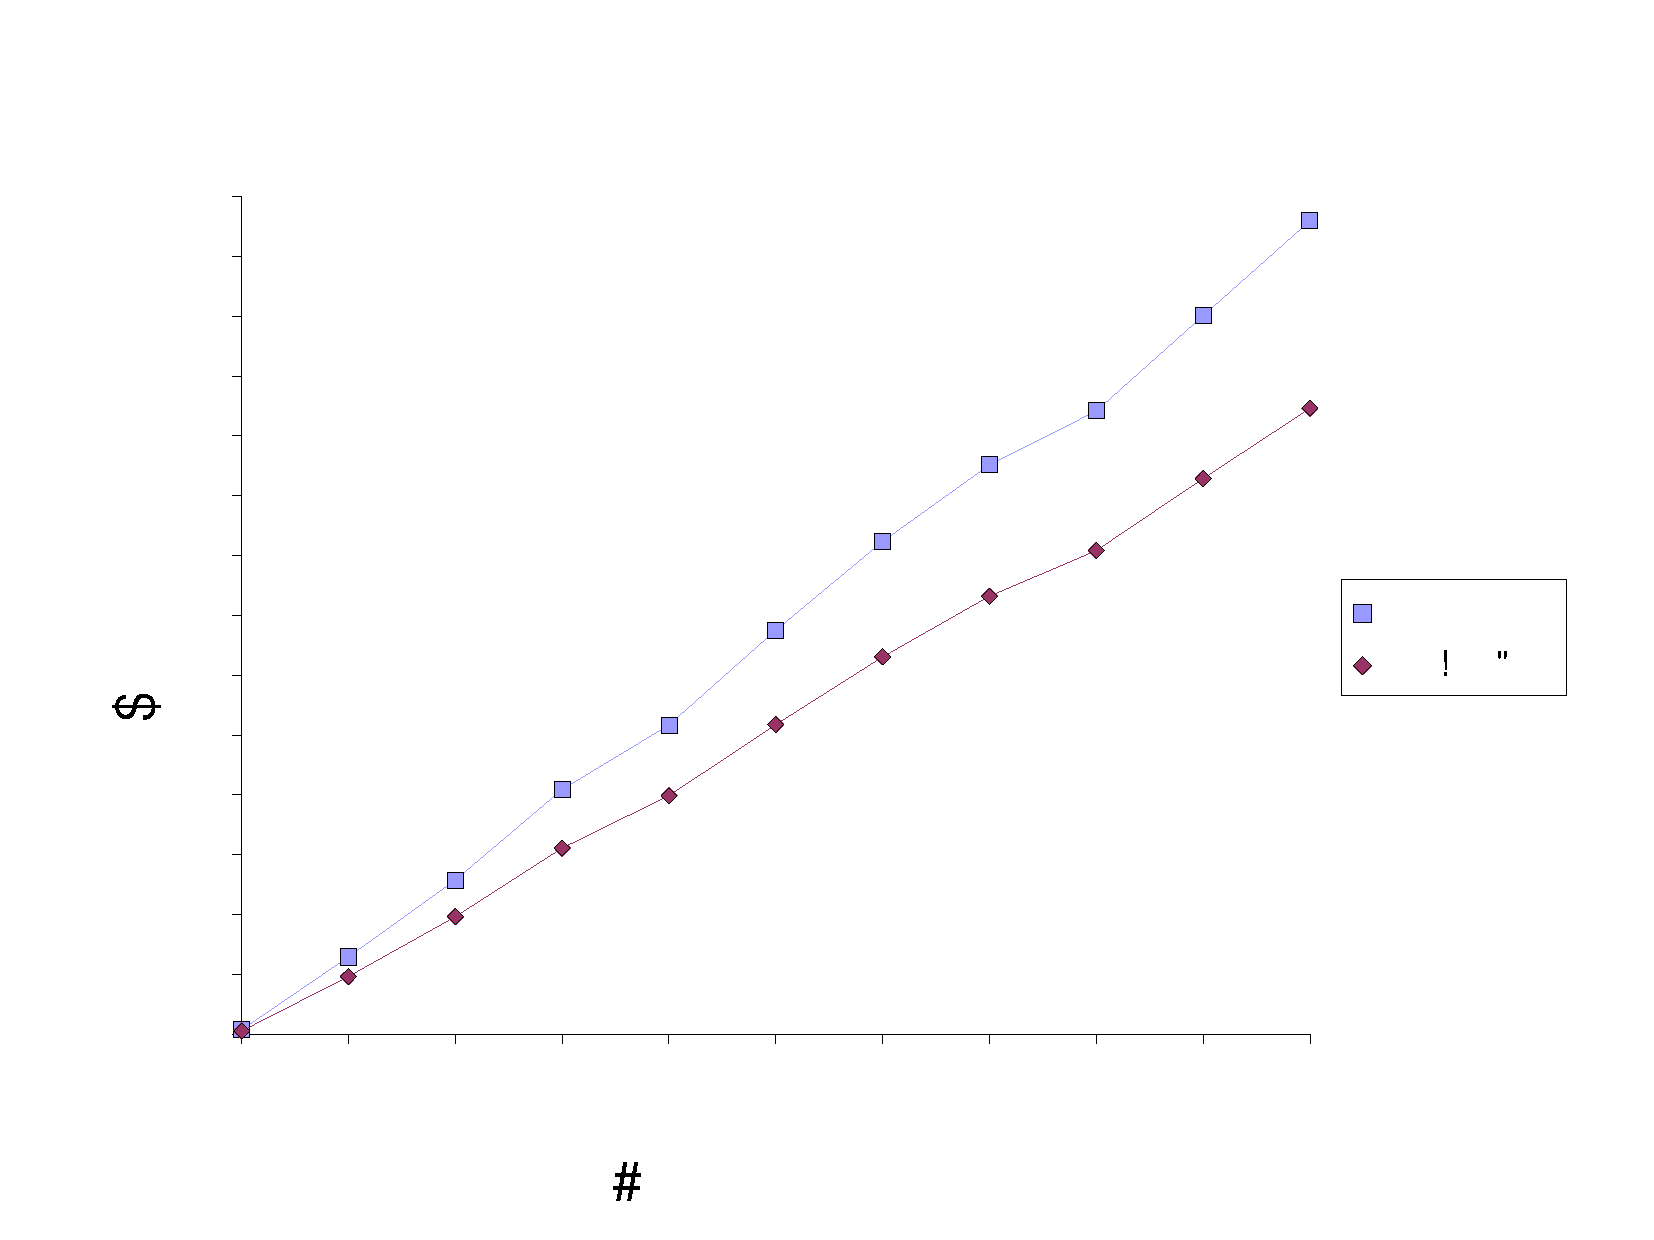
\includegraphics[%
   width=1\columnwidth]{hashTableReadGraph.pdf}
%\vspace{-30pt}
\caption{\sf\label{fig:read}The optimizer significantly speeds up
read only workloads.  As long as the data being accessed fits in page
cache, these workloads are CPU bound.  Therefore, although we report
CPU time here, these numbers are indicative of overall
performance. Figure~\ref{fig:write} explains why CPU time (and not
wall-clock time) is reported. }

\end{figure*}

In order to evaluate the performance of the optimized code, we ran
optimized and unoptimized benchmarking software on identical
workloads.  The current version of our optimizer performs a
whole-program analysis, and produces a single C source file from Cil's
internal representation.  This presents a number of problems for
performance evaluations.  First, Cil's transformation could change the
performance characteristics of the code (for the better or worse).
Second, since gcc is invoked with on a single compilation unit, it has
more opportunities to perform optimizations involving code that
originally spanned multiple compilation units.  To negate these
effects, the unoptimized versions of the benchmarks were run through
Cil without applying any \yad specific optimizations.  Both versions
of the code were then compiled using the command ``gcc -O3 input.c
-lpthread -lm -lcheck''.  For pragmatic reasons, the numbers presented
in this section reflect the code with all dynamic checks in
place.\footnote{As mentioned in Section~\ref{instrumenting}, we were
not able to run Blast directly on an executable version of the code.
We have not yet produced the (one to one) mapping between call sites
in the version processed by Blast, and in the executable version.}

Read only operations do not generate any log entries under \yad, and
largely consist of calling \pin and \unpin, and using memcpy() and
pointer arithmetic to unmarshall information stored in the page file.
Therefore, we expected \pin and \unpin to account for a significant
fraction of the runtime.  Figure~\ref{fig:read} confirms that this is
the case.

The raw read workload uses low level (page, slot, slot) recordid
triples to perform a linear scan over the page file.  This is
basically a ``best case'' scenario for the optimizer, as the top level
loop contains recordids that can be coupled to page pointers, and
current recordids are good predictors of pages that will be associated
with future recordids.  Here we see that the runtime of the optimized
version is less than half that of the original code.

The hash table workload accesses hashtable keys in sorted order,
producing random accesses to the page file.  Naively, we should not
expect the optimization to improve matters at all in this case.
However, we see that the optimized version completes in roughly 77\%
of the time the original version takes.  The reason for this
improvement is that the hashtable implementation must access a small
amount of metadata in order to service each read.  The metadata
consists of a header field, which describes the hash table and an
index page that describes the layout of the hashtable's bucket list.
The optimizer is able to take advantage of this, improving the
hashtable workload's performance.

\begin{figure*}[t]
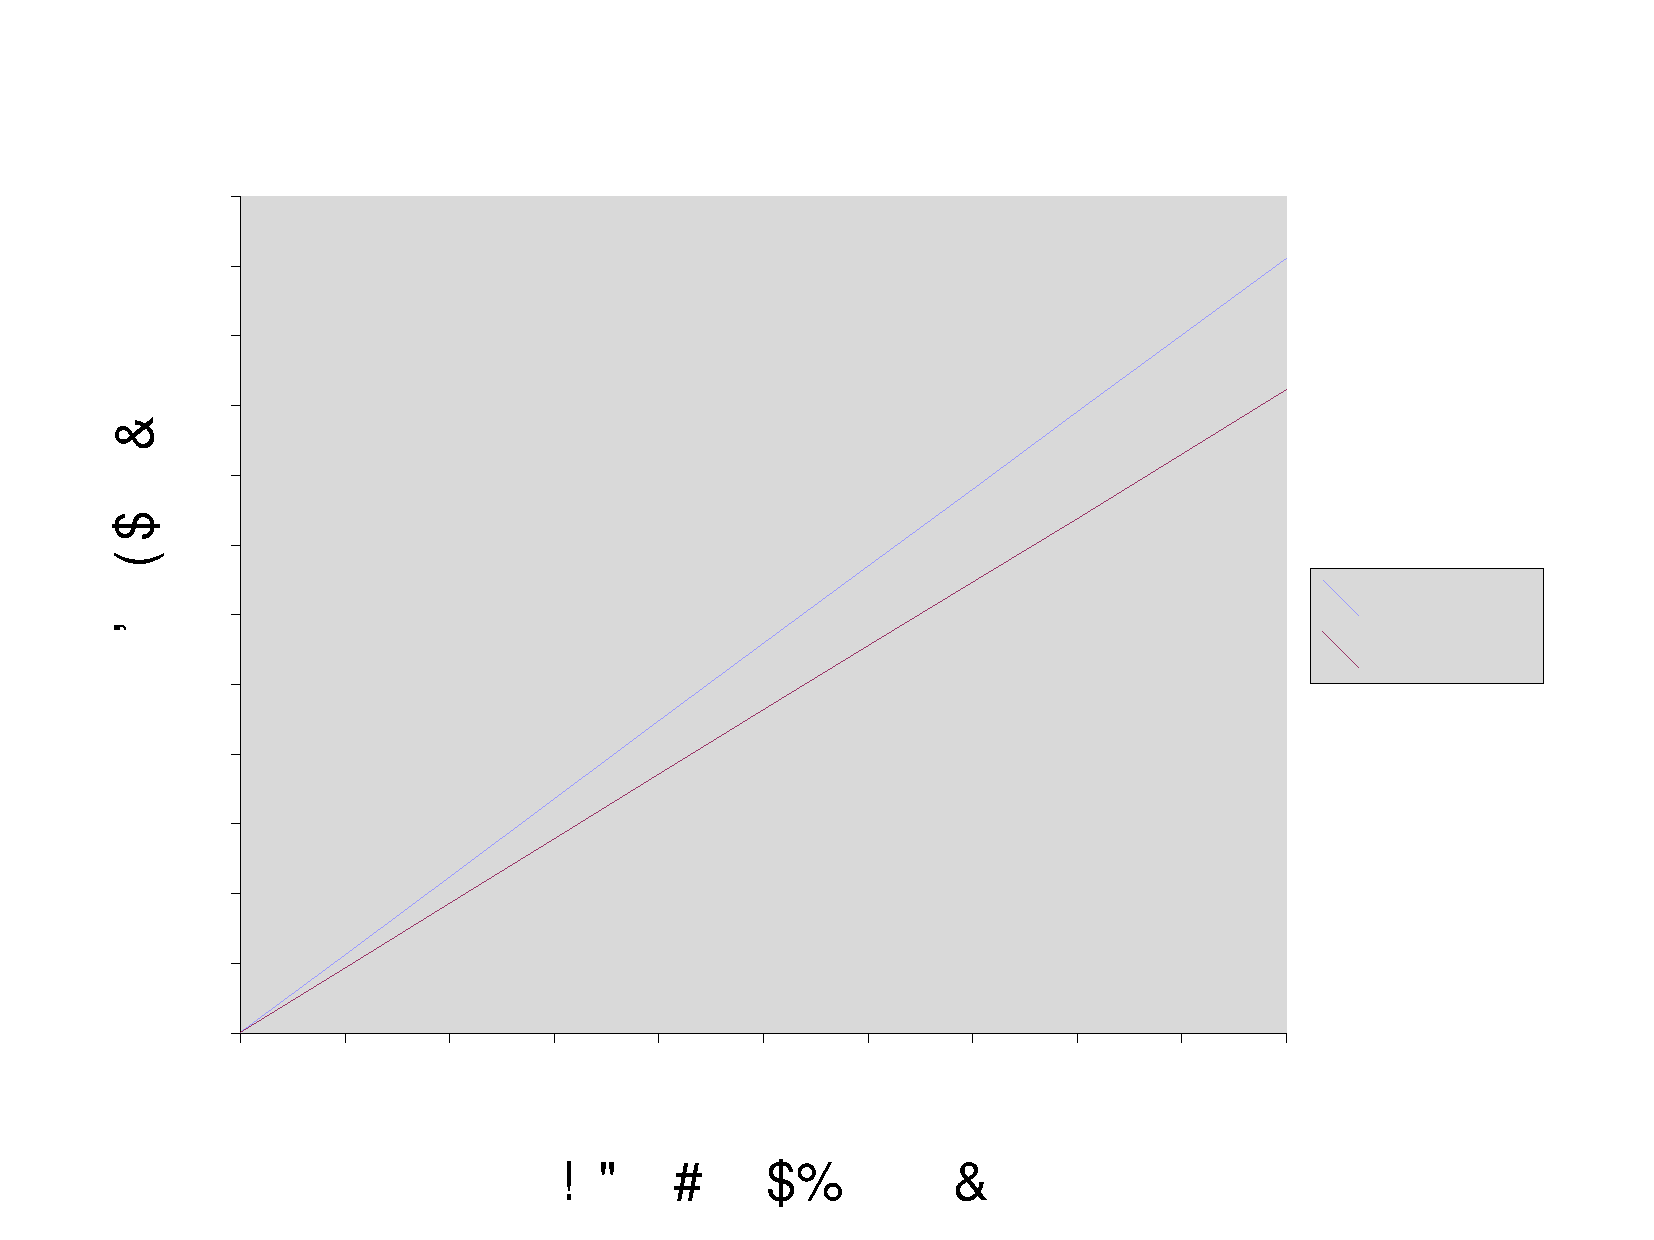
\includegraphics[%
   width=1\columnwidth]{rawWriteGraph.pdf}
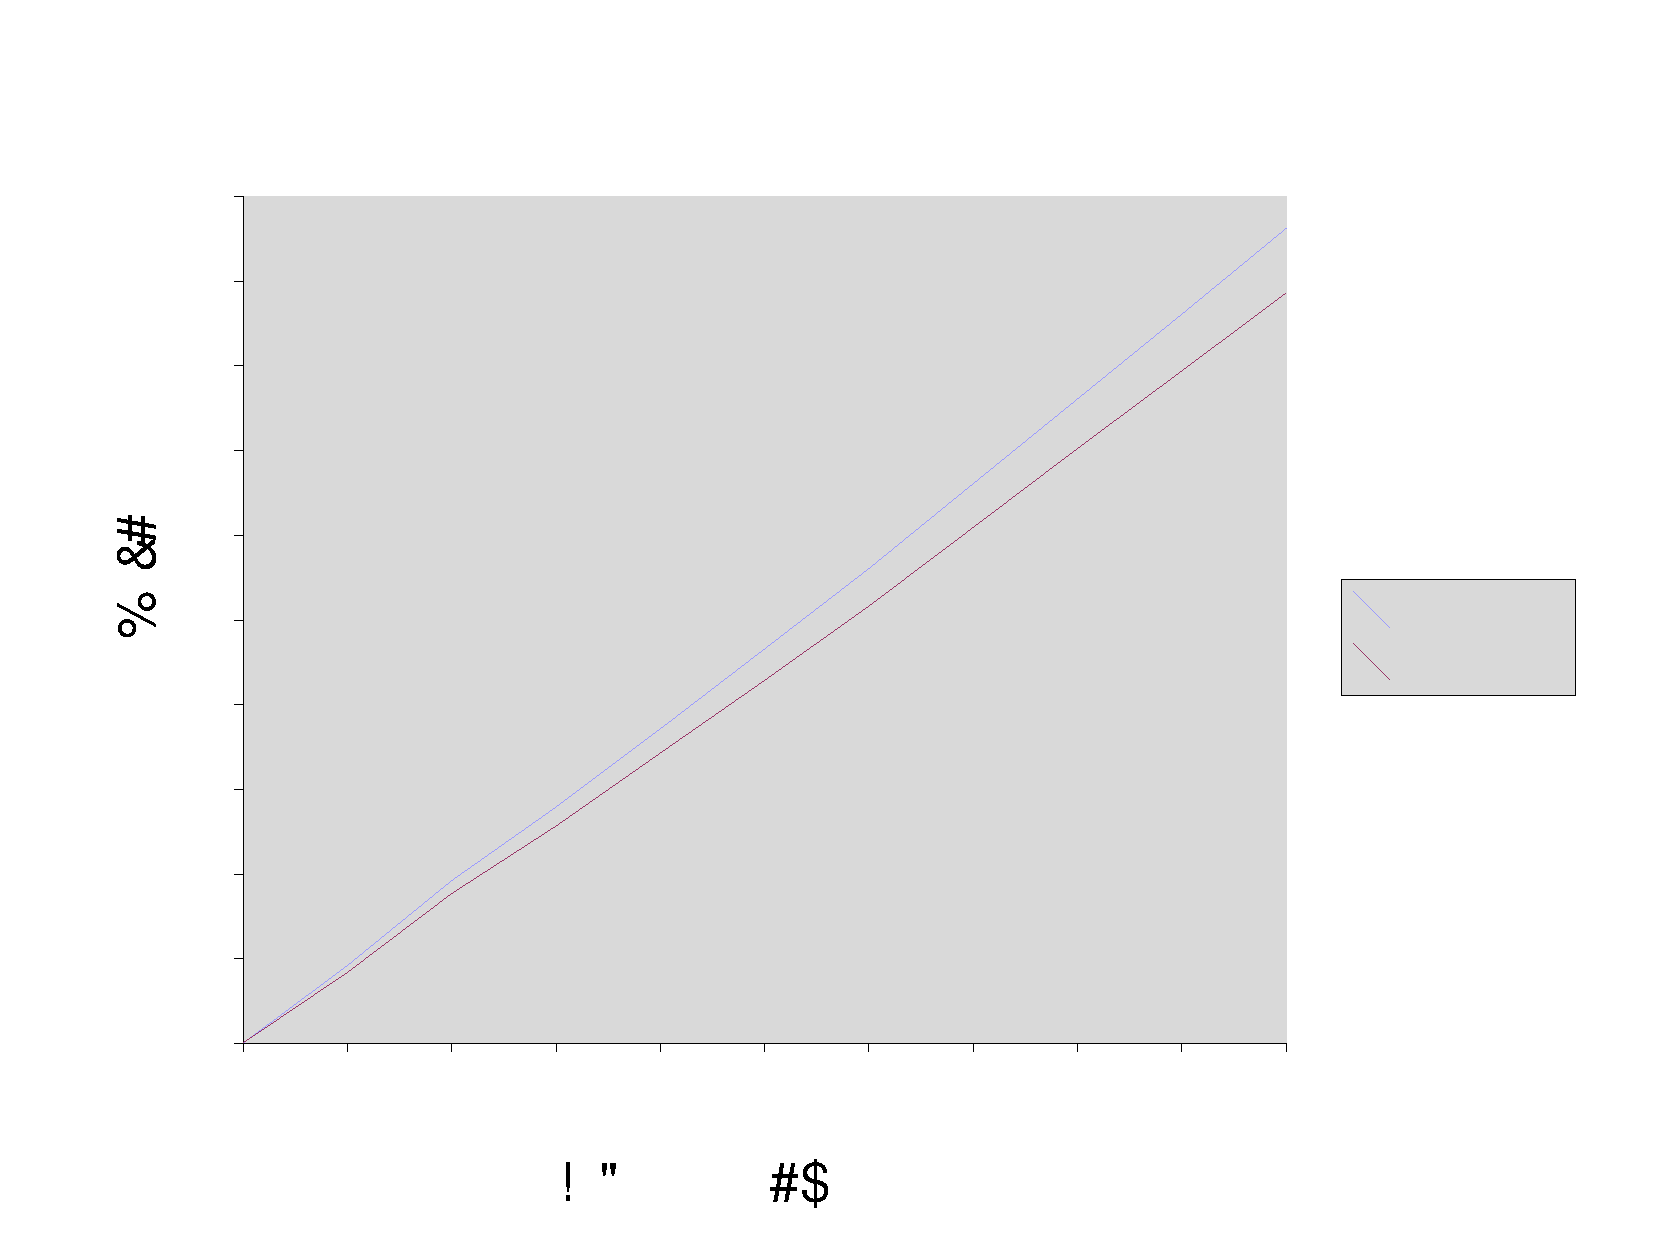
\includegraphics[%
   width=1\columnwidth]{hashTableWriteGraph.pdf}
%\vspace{-30pt}
\caption{\sf\label{fig:write}CPU times for write-only work loads.
These workloads invoke the logging subsystem, and therefore spend a
smaller fraction of their time calling \pin and \unpin.  Furthermore,
these workloads are disk bound, so wall clock times did not show any
measurable improvement in performance.  Therefore, CPU times are reported
here.  To facilitate comparison between the two workloads, CPU time is
also presented in Figure~\ref{fig:read}.}

\end{figure*}

Unfortunately, while the optimizer improves the CPU utilization of
write-only workloads, these workloads are I/O bound, so the
improvement in CPU utilization does not cause a significant improvement
in execution time.  However, the benchmark workloads do not contain
any application logic.  Therefore, CPU intenstive applications built
on top of \yad may become CPU bound even if they are write-intensive,
and will probably include a mixture of reads and writes.  Also,
multi-threaded transactional applications are able to amortize I/O
costs, so optimizations in this case are not wholly without merit.

We can see that the reduction in CPU time in the write-only case is
less than the reduction in the read-only case.  This is probably due
to the CPU overhead of the logging api, and other overhead associated
with performing logical operations in \yad. 



\subsection{Number of dynamic checks removed by Blast}

\begin{figure*}[t]
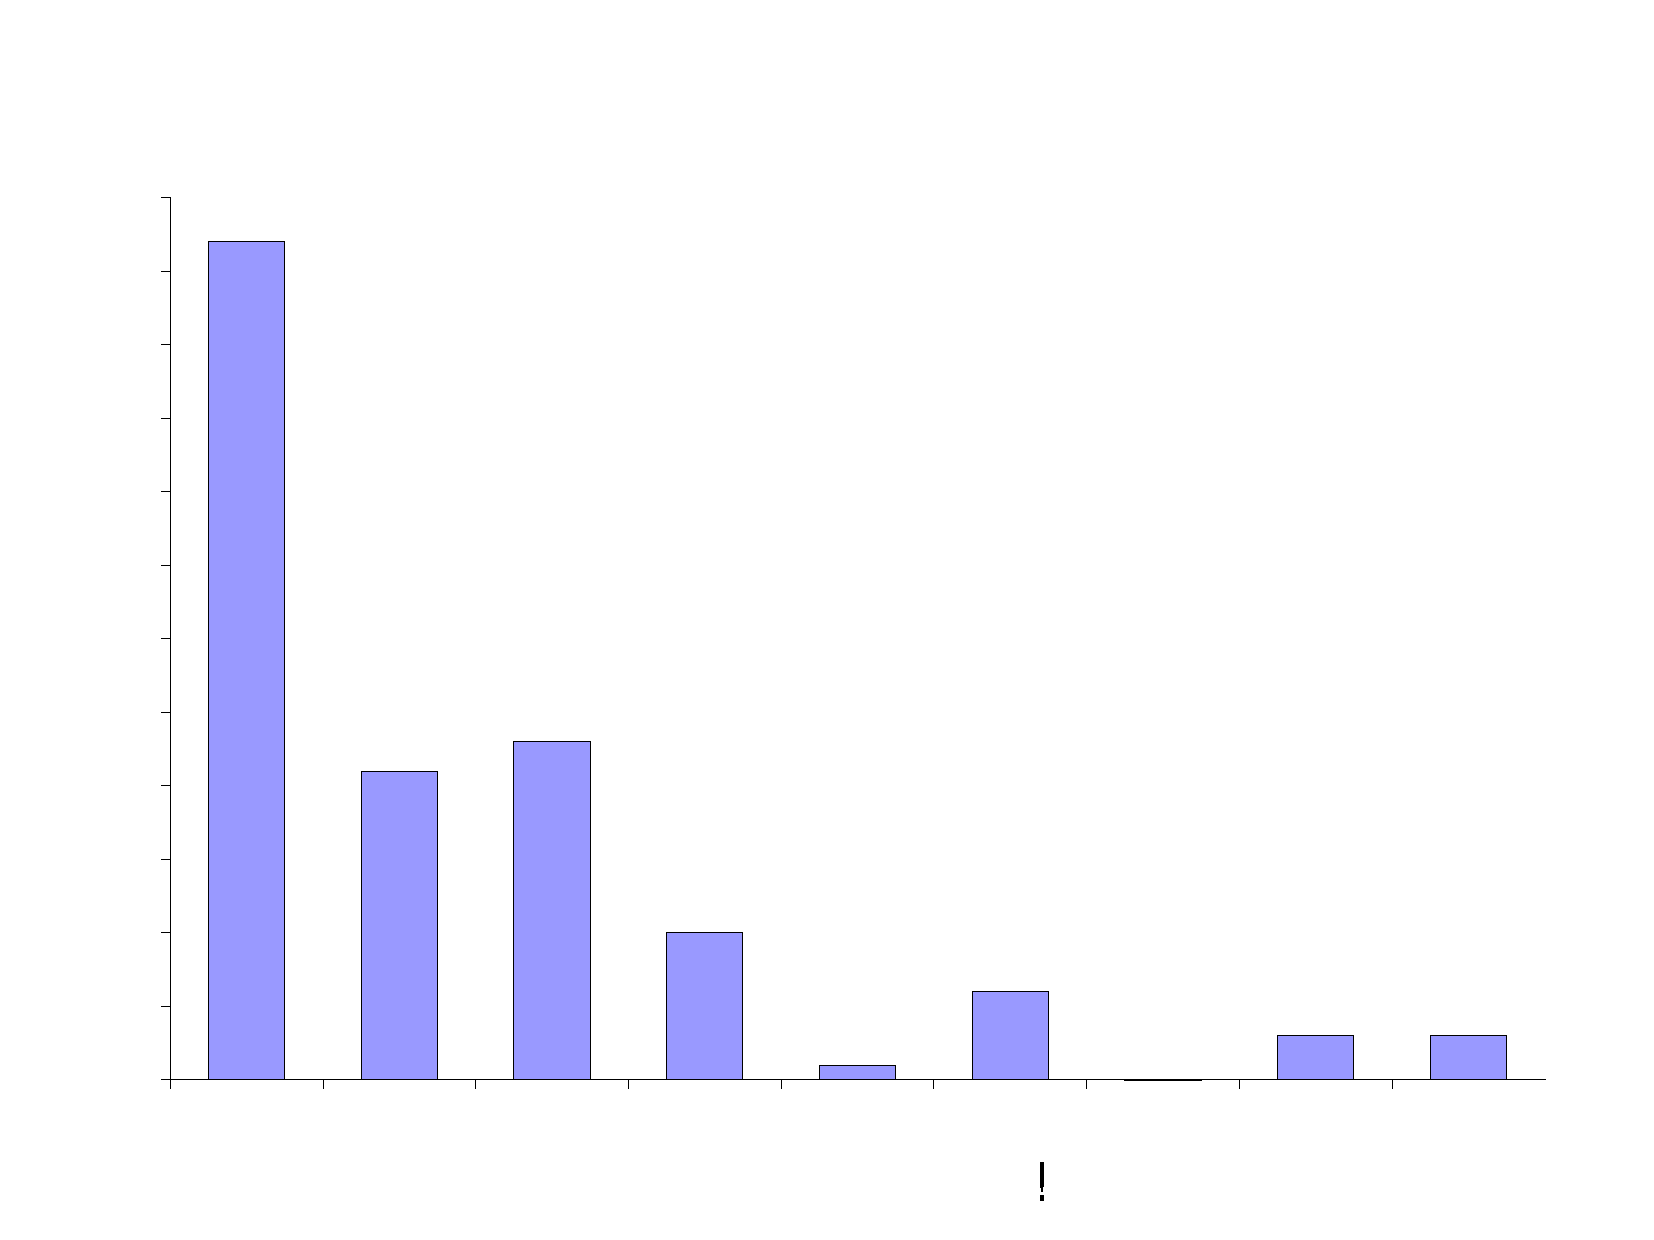
\includegraphics[%
   width=1\columnwidth]{checksRemaining.pdf}
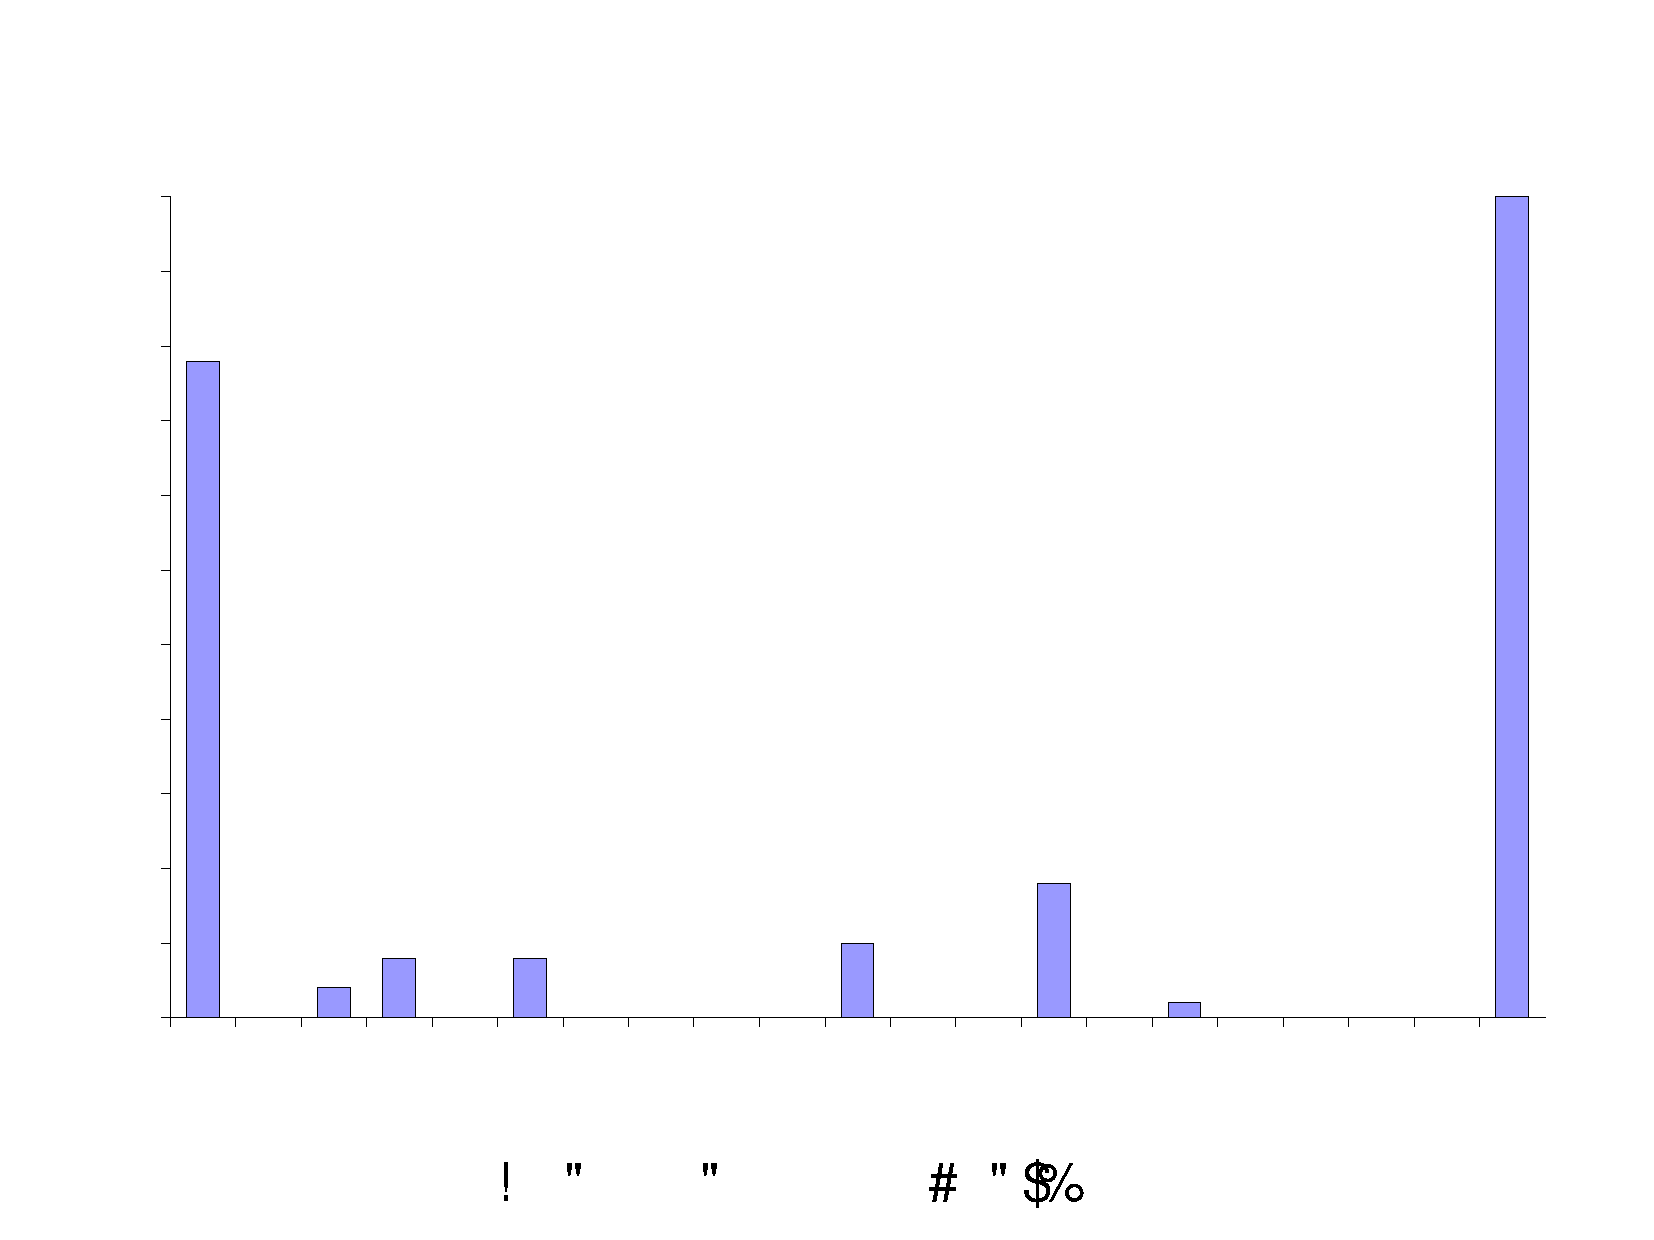
\includegraphics[%
   width=1\columnwidth]{checksRemoved.pdf}
\caption{\sf\label{fig:static}Effectiveness of naive search at
removing dynamic checks from the optimized code.  These figures include the
removal of dynamic checks and changes of calls from \fP to \fQ
variants.  These figures only include changes made during iterative
runs of Blast and only reflect checks that were actually
considered for removal.  The ignored changes and checks consist of
238 calls that were changed from \fP to \fQ variants during
preprocessing and another 238 dynamic checks that were explicitly
ignored during static checking.  Also, the system currently does not
consider dynamic checks that protect \unpin calls.}
\end{figure*}

\section{Future Work}
Although we did not begin implementing the optimizations presented in
this paper with a particular framework in mind, we believe that we
have identified a number of important properties that allow this sort
of optimization to be implemented.  Ideally, we would like to encode
these properties in a higher level language, allowing this class of 
optimization to be implemented as a simple discription of an API's properties.

In particular, optimizations geared at memoizing a function require
(1) a tight coupling between function parameters and return values,
(2) immutability of the memoized result and (3) the ability to distinguish
between a small set of variables that may be passed into the function,
and those that may not.

The first point is an obvious prerequisite of any memoization
optimziation that relies upon function arguments to retrieve cached
results.  

The second point is a bit more subtle, as it could be
achieved in at least two ways.  In our case, the ``interesting'' part of the
memoized result is the id field.  Even
though this field is not immutable over an entire program run, it is
guaranteed to be immutable until \unpin is called.  If the return
value truely is immutable over an entire program run, then the
complexities caused by \unpin could be avoided.

Finally, we used calling conventions and naming conventions to
distinguish between {\em pageid}'s and other types of variables.  The
pageid type does not explcitly exist within \yad's API.  Instead, we
used heuristics to infer its type.  In other circumstances the API
might provide rich enough type information to avoid inference
entirely, or a type inference system such as Cqual might be more
appropriate.

It may be possible to generalize our system so that it can handle all
of these scenarios.  Such a generalized system seems to be sufficient
to support general purpose, high-level definitions of automated
memoization transformations.

Along these lines, we have mentioned a few other potential approaches
toward storing memoized results throughout this paper.  One idea that
occurred to us but that would be difficult to implement for \yad
maintains static, per function (or per call-site) Page pointers.  The
Page pointers could store memoized results across calls to the
function, and this persistant information could be used in addition to to
the \PP parameter.

The difficulty in implementing this scheme arises because it becomes
unclear how and when \unpin should be called, since static pointers
could persist indefinitely.  In systems that
memoize idempotent return values, this would not be an issue, since
these systems would not contain a call that is analagous to \unpin.

In \yad's case, it should be possible to 'partially release' a page by
calling \unpin, but keeping a copy of the page pointer.  Before making
an expensive call to \pin the function could speculatively latch
whatever the partially released pointer points
to.\footnote{\yad would guarantee that it points to a valid Page
struct} If the pointer still points to the desired page, this
scheme would avoid an expensive hashtable lookup.

% - improve quality of transformation
% - add optimizations for other calls (Tread)
% - allow for higher level definitions of this type of transformation (outline high-level principles here)
% - look at other applications for the technique
% - provide mechanism to transform / optimize library once, and then use information from library tranformation while transforming client code.
\section{Conclusion}

We have designed and implemented a C source to source translation that
implements high-level, application specific optimizations.  Such
systems are currently uncommon, but we argue that modern programming
practices greatly increase their importance.  We validate this claim
by showing that our optimization technique significantly increases the
performance of an existing library.  We are unaware of any other
systems that take our approach toward program optimization.  We
believe that our use combination of aggressive optimization techniques
and conservative runtime checks is particularly valuable.  The use of
a general purpose tool to reduce the overhead associated with runtime
checks reduces the overhead associated with these techniques.  This
makes it easier to implement a wide variety of application-specific
optimization techniqes that probably would not be worth the
development effort if implemented from scratch.  Finally, we believe
that by moving the implementation of complex optimization techniques
to compile time, our system improves the maintainability of software
without sacrificing performance.

\begin{thebibliography}{99}
\begin{small}
\bibitem[1]{multipleGenericLocking} Agrawal, et al. {\em Concurrency
Control Performance Modeling: Alternatives and Implications}. TODS
12(4): (1987) 609-654

%\bibitem[2]{bdb} Berkeley~DB, {\tt http://www.sleepycat.com/}

%\bibitem[3]{capriccio} R. von Behren, J Condit, F. Zhou, G. Necula, and E. Brewer. {\em Capriccio: Scalable Threads for Internet Services} SOSP 19 (2003).

\bibitem[2]{oo7} Carey, Michael J., DeWitt, David J., Naughton, Jeffrey F. {\em The OO7 Benchmark.} SIGMOD (1993)

\bibitem[3]{relational} E. F. Codd, {\em A Relational Model of Data for Large Shared Data Banks.} CACM 13(6) p. 377-387 (1970)

\bibitem[4]{mapReduce} Jeffrey Dean and Sanjay Ghemawat. {\em Simplified Data Processing on Large Clusters. } OSDI (2004)

%\bibitem[5]{lru2s} Envangelos P. Markatos. {\em On Caching Search Engine Results}.  Institute of Computer Science, Foundation for Research \& Technology - Hellas (FORTH) Technical Report 241 (1999)

\bibitem[5]{soft-updates} Greg Ganger.  {\em Soft Updates: A Solution to the Metadata Update Problem in File Systems } ACM Transactions (2000)

\bibitem[6]{semantic} David K. Gifford, P. Jouvelot, Mark A. Sheldon, and Jr. James W. O'Toole. {\em Semantic file systems}. Proceedings of the Thirteenth ACM Symposium on Operating Systems Principles, (1991) p. 16-25.

\bibitem[7]{physiological} Gray, J. and Reuter, A. {\em Transaction Processing: Concepts and Techniques}. Morgan Kaufmann (1993) San Mateo, CA

\bibitem[8]{hierarcicalLocking} Jim Gray, Raymond A. Lorie, and Gianfranco R. Putzulo. {\em Granularity of locks and degrees of consistency in a shared database}. In 1st International Conference on VLDB, September 1975. Reprinted in Readings in Database Systems, 3rd ed.

\bibitem[9]{cht}  Gribble, Steven D., Brewer, Eric A., Hellerstein, Joseph M., Culler, David.  {\em Scalable, Distributed Data Structures for Internet Service Construction. } OSDI (2000)

\bibitem[9]{haerder} Haerder \& Reuter {\em "Principles of Transaction-Oriented Database Recovery." } Computing Surveys 15(4) (1983) % p 287-317

\bibitem[10]{hibernate} Hibernate, {\tt http://www.hibernate.org/}

\bibitem[11]{lamb} Lamb, et al., {\em The ObjectStore System.} CACM 34(10) (1991)

%\bibitem[12]{blink} Lehman \& Yao, {\em Efficient Locking for Concurrent Operations in B-trees.} TODS 6(4) (1981) p. 650-670

\bibitem[12]{lht} Litwin, W., {\em Linear Hashing: A New Tool for File and Table Addressing}. Proc. 6th VLDB, Montreal, Canada, (Oct. 1980) % p. 212-223

\bibitem[13]{aries} Mohan, et al., {\em ARIES: A Transaction Recovery Method Supporting Fine-Granularity Locking and Partial Rollbacks Using Write-Ahead Logging.} TODS 17(1) (1992) p. 94-162

\bibitem[14]{twopc} Mohan, Lindsay \& Obermarck, {\em Transaction Management in the R* Distributed Database Management System} TODS 11(4) (1986) p. 378-396

\bibitem[15]{ariesim} Mohan, Levine. {\em ARIES/IM: an efficient and high concurrency index management method using write-ahead logging} International Converence on Management of Data, SIGMOD (1992) p. 371-380

\bibitem[16]{mysql} {\em MySQL}, {\tt http://www.mysql.com/ }

\bibitem[17]{reiser} Reiser,~Hans~T. {\em ReiserFS 4} {\tt http://www.namesys.com/ }
%
\bibitem[18]{berkeleyDB} M. Seltzer, M. Olsen. {\em LIBTP: Portable, Modular Transactions for UNIX}. Proceedings of the 1992 Winter Usenix (1992)

\bibitem[19]{lrvm} Satyanarayanan, M., Mashburn, H. H., Kumar, P., Steere, D. C., AND Kistler, J. J. {\em Lightweight Recoverable Virtual Memory}. ACM Transactions on Computer Systems 12, 1 (Februrary 1994) p. 33-57. Corrigendum: May 1994, Vol. 12, No. 2, pp. 165-172.

\bibitem[20]{newTypes} Stonebraker. {\em Inclusion of New Types in Relational Data Base. } ICDE (1986) %p. 262-269

\bibitem[21]{postgres} Stonebraker and Kemnitz. {\em The POSTGRES Next-Generation Database Management System. } CACM (1991)

%\bibitem[SLOCCount]{sloccount} SLOCCount, {\tt http://www.dwheeler.com/sloccount/ }
%
%\bibitem[lcov]{lcov} The~LTP~gcov~extension, {\tt http://ltp.sourceforge.net/coverage/lcov.php }
%


%\bibitem[Beazley]{beazley} D.~M.~Beazley and P.~S.~Lomdahl, 
%{\em Message-Passing Multi-Cell Molecular Dynamics on the Connection
%Machine 5}, Parall.~Comp.~ 20 (1994) p. 173-195.
%
%\bibitem[RealName]{CitePetName} A.~N.~Author and A.~N.~Other, 
%{\em Title of Riveting Article}, JournalName VolNum (Year) p. Start-End
%
%\bibitem[ET]{embed} Embedded Tk, \\
%{\tt ftp://ftp.vnet.net/pub/users/drh/ET.html}
%
%\bibitem[Expect]{expect} Don Libes, {\em Exploring Expect}, O'Reilly \& Associates, Inc. (1995).
%
%\bibitem[Heidrich]{heidrich} Wolfgang Heidrich and Philipp Slusallek, {\em
%Automatic Generation of Tcl Bindings for C and C++ Libraries.},
%USENIX 3rd Annual Tcl/Tk Workshop (1995).
%
%\bibitem[Ousterhout]{ousterhout} John K. Ousterhout, {\em Tcl and the Tk Toolkit}, Addison-Wesley Publishers (1994).
%
%\bibitem[Perl5]{perl5} Perl5 Programmers reference,\\
%{\tt http://www.metronet.com/perlinfo/doc}, (1996).
%
%\bibitem[Wetherall]{otcl} D. Wetherall, C. J. Lindblad, ``Extending Tcl for
%Dynamic Object-Oriented Programming'', Proceedings of the USENIX 3rd Annual Tcl/Tk Workshop (1995).
\end{small}
\end{thebibliography}



\end{document}

